\documentclass{standalone}
\usepackage{tikz}
\begin{document}
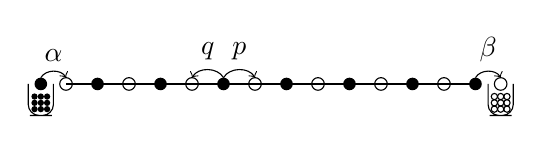
\begin{tikzpicture}[scale=0.8]
  % Draw the line
  \draw[thick] (-0.5,0) -- (6,0);

  % Draw the lattice sites
  \foreach \x in {-0.5, 0.5, ..., 5.5}
    \draw (\x,0) circle (0.1cm);

  % Draw the occupied sites
  \foreach \x in {0, 1, ..., 6}
    \fill (\x,0) circle (0.1cm);

  % Draw the reservoirs
  \draw[rounded corners] (-1.1,0) |- (-0.9,-0.5) -| (-0.7,0);

  \draw[rounded corners] (6.2,0) |- (6.4,-0.5) -| (6.6,0);

  % Draw a few smaller particles in the reservoirs
    \foreach \x in {-0.8, -0.9, -1}
    \foreach \y in {-0.2, -0.3, -0.4}
      \fill (\x,\y) circle (0.05cm);

    \foreach \x in {6.5, 6.4, 6.3}
    \foreach \y in {-0.2, -0.3, -0.4}
      \draw (\x,\y) circle (0.05cm);

    % draw one big particle in the reservoirs
    \fill (-0.9,0) circle (0.1cm);
    \draw (6.4,0) circle (0.1cm);

    % draw the arrows
    \path (2,0.1) edge[->,bend left=60] node[above] {$p$} (2.5,0.1);
    \path (2,0.1) edge[->,bend right=60] node[above] {$q$} (1.5,0.1);

    \path (-0.9,0.1) edge[->,bend left=60] node[above] {$\alpha$} (-0.5,0.1);
    \path (6.0,0.1) edge[->,bend left=60] node[above] {$\beta$} (6.4,0.1);






\end{tikzpicture}
\end{document}
